\documentclass{scrartcl}
\usepackage[utf8]{inputenc}
\usepackage[spanish,es-tabla]{babel}	% Paquete de idiomas 'babel':
						%
						% 	Idioma: 'spanish'
						%	Opciones:
						%		es-tabla: sustituye la palabra 'cuadro' por 'tabla'.

\usepackage{amsmath,amsfonts,amsthm}
\usepackage{txfonts}	% Fuente Times
\renewcommand{\sectfont}{\rmfamily \bfseries} %cabeceras y titulos con estilo roman, negrita.


\usepackage{booktabs}	% Permite construir tablas de alta calidad.
\usepackage{tabu}
\usepackage{caption}
\usepackage{subcaption}
\usepackage{hyperref}
\usepackage{txfonts}
\usepackage{notoccite}
\usepackage{xspace}

\usepackage[thinspace,mediumqspace,squaren]{SIunits}	% Sistema Internacional de unidades.
	\newcommand{\micras}{\micro\meter\xspace}
	\newcommand{\mm}{\milli\meter\xspace}
	\newcommand{\cm}{\centi\meter\xspace}
	\newcommand{\nm}{\nano\meter\xspace}

	\newcommand{\Exp}[1]{\cdot\power{10}{#1}}
	\newcommand{\vect}[1]{\mathbf{#1}}

%% TikZ %%
%
\usepackage{tikz}
\usepackage{pgfplots}
\pgfplotsset{compat=1.3}


\usepackage{float}
\newfloat{grafica}{htbp}{log}
\floatname{grafica}{Gráfica}


%% TikZ %%
%
\usepackage{tikz}


\renewcommand{\thesubsection}{\thesection.\alph{subsection}}
\usepackage[makeroom]{cancel}

\title{Estadística - Hoja 1}
\author{Ignacio Suárez Andrés}
\date{1 de diciembre de 2014}

\begin{document}
\maketitle

\section{Determinación de $T_c$}
Para conocer qué valores de $T$ tiene sentido analizar, conviene determinar primero la temperatura crítica. Con este fin, partimos de dos valores, $T=1$ y $T=3$ que comprobamos fácilmente que corresponden a los comportamientos ferromagnético y paramagnético respectivamente.\par
Recorremos los valores intermedios en intervalos de $\Delta T = 0.005$, realizando para cada uno una simulación con 20000 pasos de tiempo y extrayendo de cada una el promedio y la desviación estándar de la magnetización media del sistema, midiendo ésta en los últimos 10000 pasos. Se muestran los resultados en la figura \ref{fig:allT}, de donde se pueden extraer las siguientes conclusiones:\par
\begin{itemize}
\item Existe una temperatura crítica $T_c \approx$ 2,3 por debajo de la cual se da el comportamiento ferromagnético, con todos los spines tendiendo a orientarse en el mismo sentido, y por encima de la cual el comportamiento es paramagnético, con magnetización promedio aproximadamente nula.
\item La forma de la gráfica se corresponde con una bifurcación horquilla (o \textit{pitchfork}) supercrítica.
\item De las simulaciones con magnetización media mayor que 0,95 en valor absoluto, el 47\% (150) tienen valor positivo y el 53\% (168) negativo, valores cercanos al 50\% esperado. Se forman también, con $T<T_c$ estados en los que se forman dominios magnéticos y no llegan a tender a uno de los dos extremos, aunque sus fluctuaciones muestran que no son estables.
\item Las temperaturas altas dificultan la formación de pequeños dominios, reduciendo así cada vez más la probabilidad de alejarse del valor 0 mediante fluctuaciones.
\end{itemize}

\begin{figure}
\centering
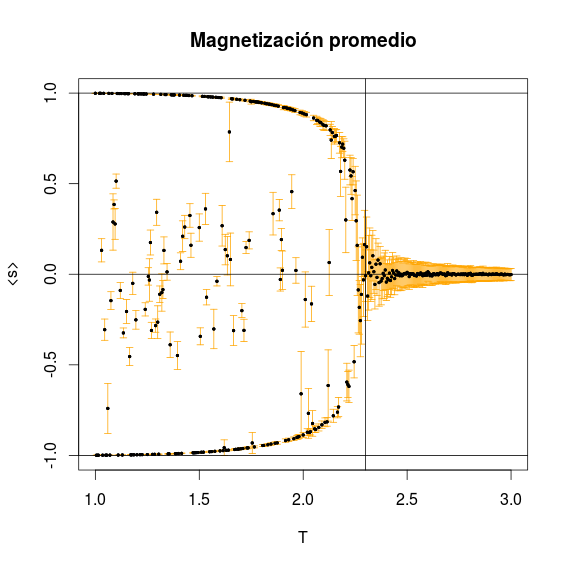
\includegraphics[scale=0.7]{allT}
\caption{Valores promedio de la magnetización para 400 valores de T, junto a la desviación estándar para representar las fluctuaciones dentro del periodo de tiempo recogido.}
\label{fig:allT}
\end{figure}




\clearpage
\section{Evolución temporal}
Para entender el efecto de la temperatura, es conveniente analizar la evolución de la magnetización media desde su inicialización aleatoria.\par
En la figura \ref{fig:tempnoTc} se han representado varios casos con temperaturas alejadas del punto crítico. Para $T<T_c$, la estabilización en torno a +1 o -1 es rápida, salvo para las excepciones en las que se forman dominios en el material. Para $T>T_c$, la magnetización media oscila cerca de 0. Se puede apreciar en ambos casos cómo la temperatura favorece el desorden, oponiéndose a la estabilización lejos de 0.
Por otra parte, en la figura \ref{fig:tempTc} se ha estudiado el comportamiento con temperaturas cercanas a $T_c$. Vemos cómo, partiendo de $T<T_c$ y subiendo, la magnetización media va dejando de estabilizarse en un valor extremo y va tomando valores menores, llegando hasta el punto de que para $T>T_c$ las oscilaciones se producen en torno a 0. Sin embargo, en torno a $T_c$, especialmente para $T=$ 2,3, las fluctuaciones se vuelven muy bruscas, pasando de golpe de estados con orientación mayoritariamente positiva a negativa y viceversa, sin alcanzar un punto de estabilizar en torno al cual oscilar.
\begin{figure}[ht]
\centering
\begin{subfigure}{.5\textwidth}
  \centering
  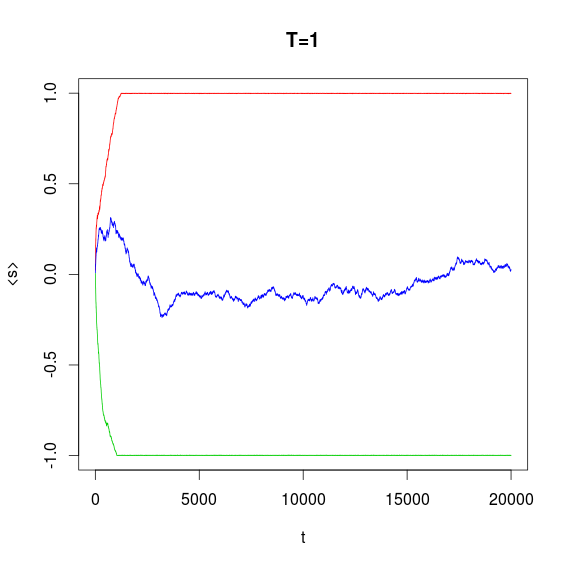
\includegraphics[width=1\linewidth]{T1}
\end{subfigure}%
\begin{subfigure}{.5\textwidth}
  \centering
  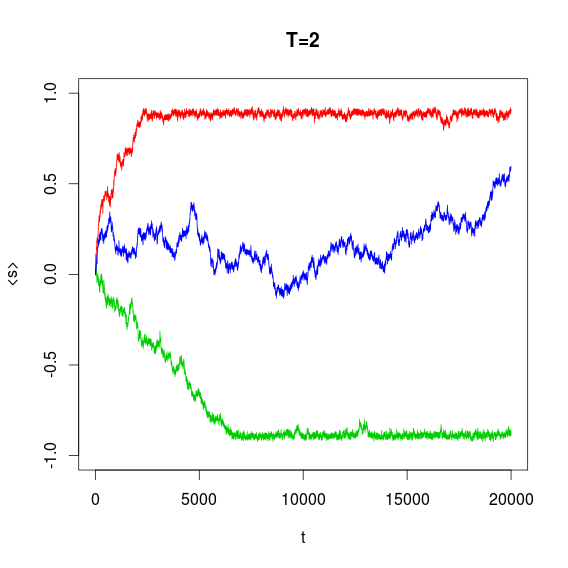
\includegraphics[width=1\linewidth]{T2}
\end{subfigure}
\begin{subfigure}{.5\textwidth}
  \centering
  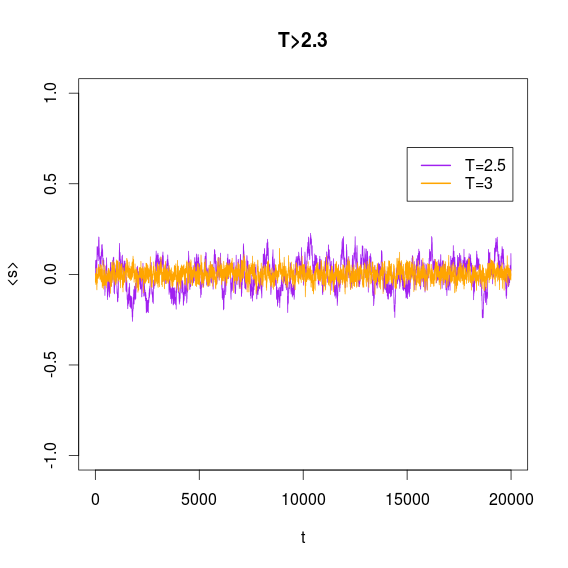
\includegraphics[width=1\linewidth]{T3}
\end{subfigure}
\caption{Evolución temporal de la magnetización media para diferentes temperaturas alejadas de $T_c$, representando en cada caso todos los comportamientos que pueden darse.}
\label{fig:tempnoTc}
\end{figure}

\begin{figure}[ht]
\centering
\begin{subfigure}{.6\textwidth}
  \centering
  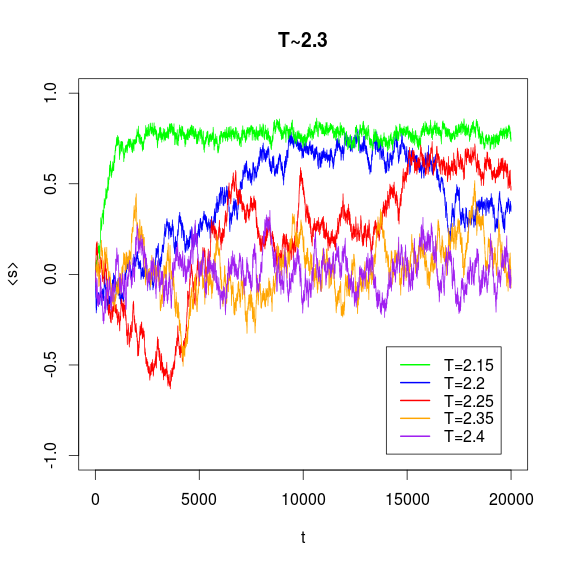
\includegraphics[width=1\linewidth]{Tno23}
\end{subfigure}
\begin{subfigure}{.6\textwidth}
  \centering
  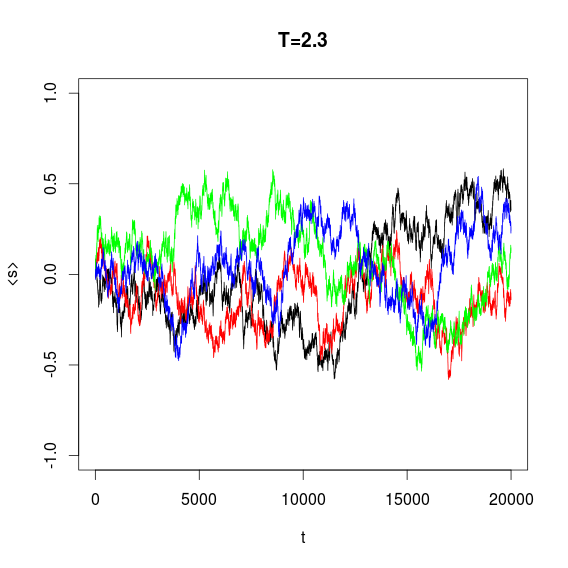
\includegraphics[width=1\linewidth]{T23}
\end{subfigure}
\caption{Evolución temporal de la magnetización media para temperaturas en torno a $T_c$, con especial detalle para $T=$ 2,3.}
\label{fig:tempTc}
\end{figure}

\clearpage
\section{Problema 3}
\begin{figure}[ht]
\centering
\begin{subfigure}{.35\textwidth}
  \centering
  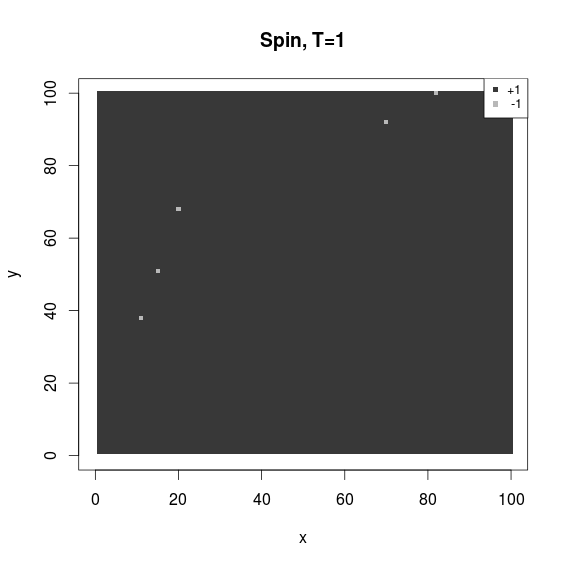
\includegraphics[width=1\linewidth]{spins/spinT1+}
\end{subfigure}%
\begin{subfigure}{.35\textwidth}
  \centering
  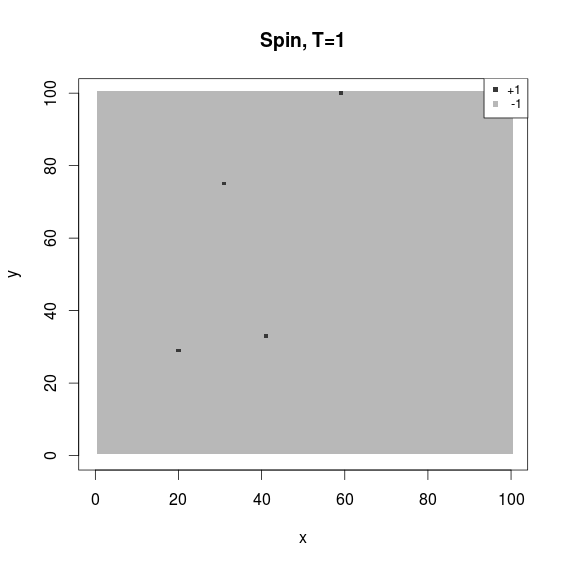
\includegraphics[width=1\linewidth]{spins/spinT1-}
\end{subfigure}%
\begin{subfigure}{.35\textwidth}
  \centering
  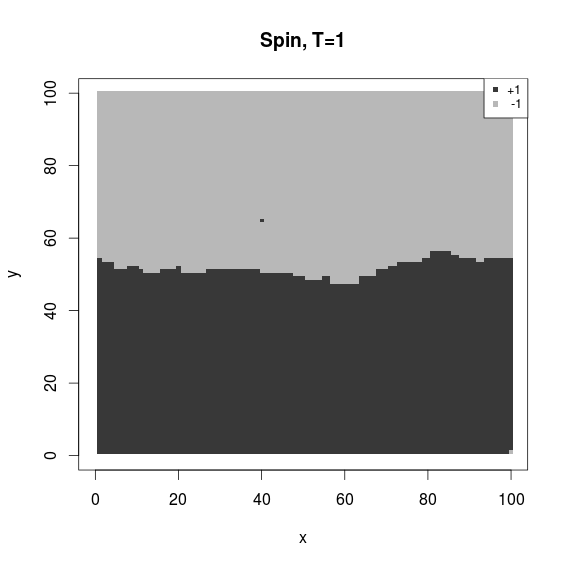
\includegraphics[width=1\linewidth]{spins/spinT1doms}
\end{subfigure}
\begin{subfigure}{.35\textwidth}
  \centering
  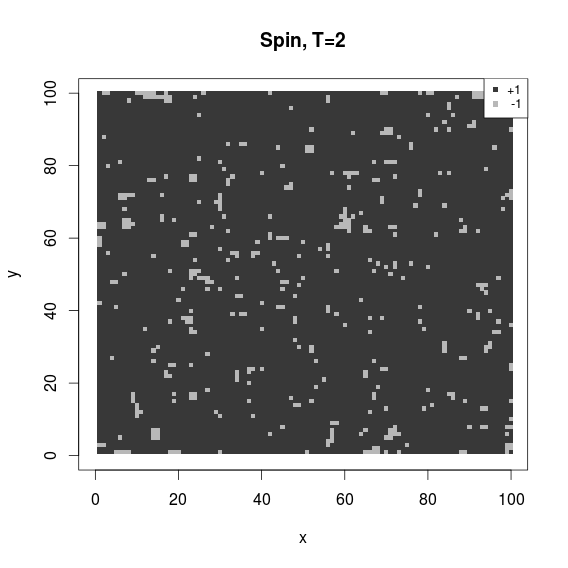
\includegraphics[width=1\linewidth]{spins/spinT2+}
\end{subfigure}%
\begin{subfigure}{.35\textwidth}
  \centering
  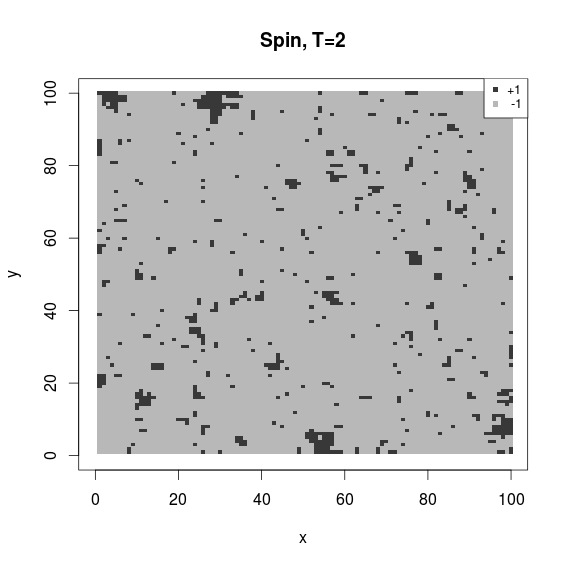
\includegraphics[width=1\linewidth]{spins/spinT2-}
\end{subfigure}%
\begin{subfigure}{.35\textwidth}
  \centering
  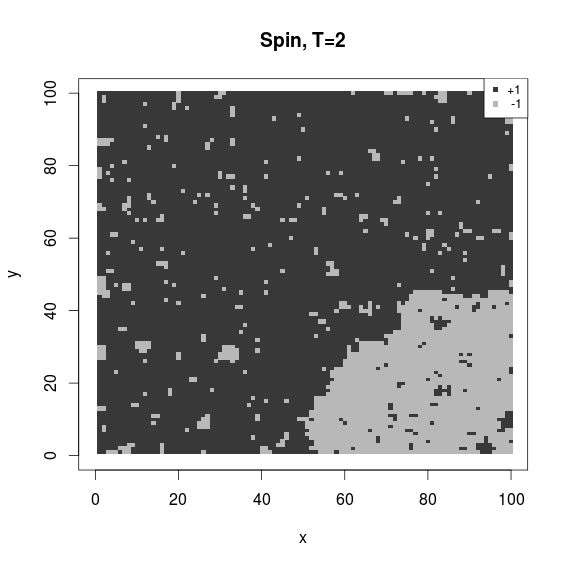
\includegraphics[width=1\linewidth]{spins/spinT2doms}
\end{subfigure}
\begin{subfigure}{.35\textwidth}
  \centering
  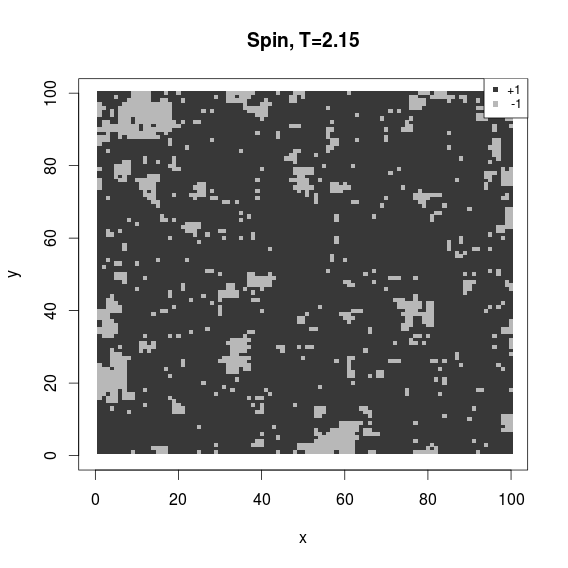
\includegraphics[width=1\linewidth]{spins/spinT2_15}
\end{subfigure}%
\begin{subfigure}{.35\textwidth}
  \centering
  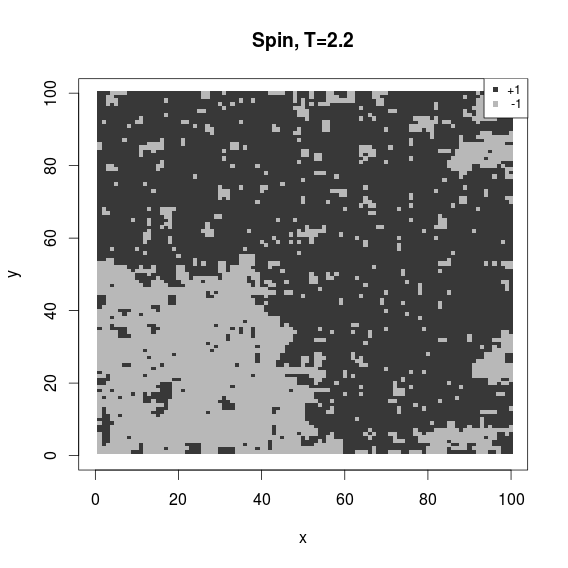
\includegraphics[width=1\linewidth]{spins/spinT2_2}
\end{subfigure}%
\begin{subfigure}{.35\textwidth}
  \centering
  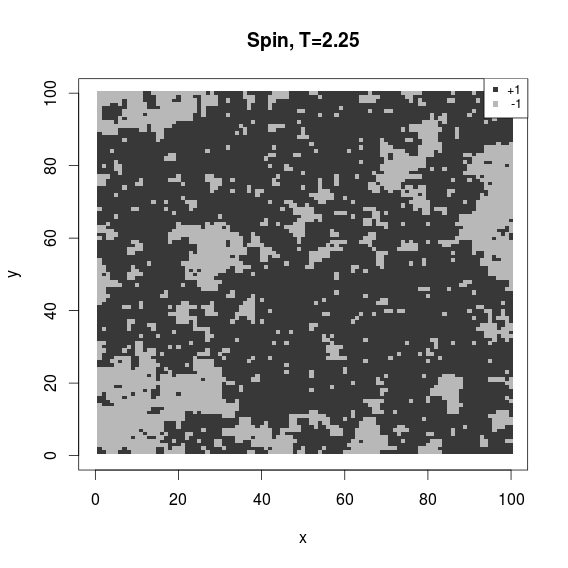
\includegraphics[width=1\linewidth]{spins/spinT2_25}
\end{subfigure}
\caption{Evolución temporal de la magnetización media para diferentes temperaturas alejadas de $T_c$, representando en cada caso todos los comportamientos que pueden darse.}
\label{fig:spinsmenorTc}
\end{figure}

\begin{figure}[ht]
\centering
\begin{subfigure}{.35\textwidth}
  \centering
  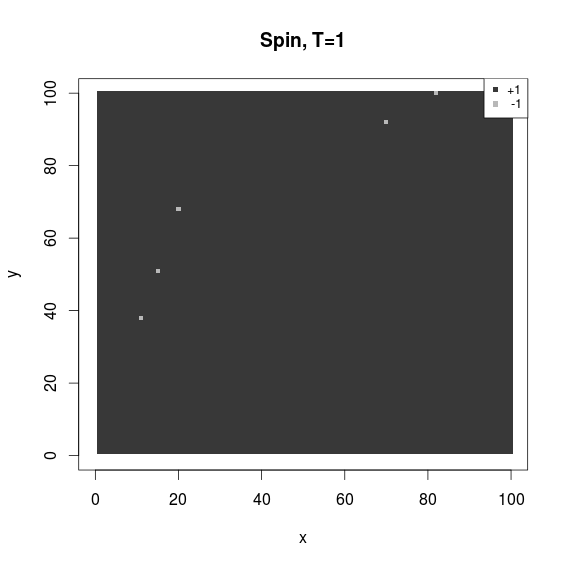
\includegraphics[width=1\linewidth]{spins/spinT1+}
\end{subfigure}%
\begin{subfigure}{.35\textwidth}
  \centering
  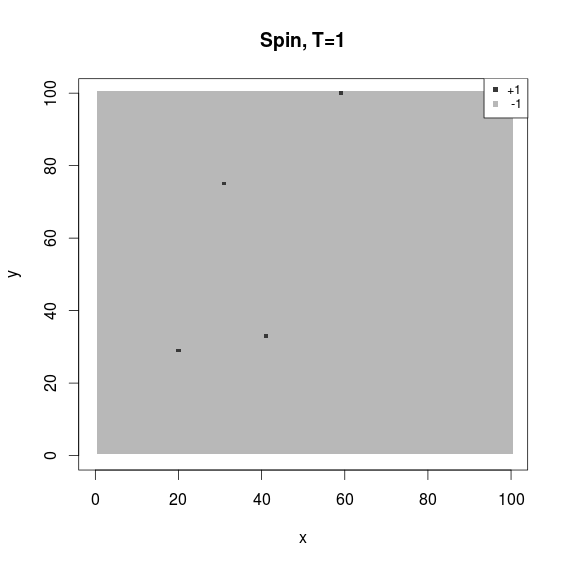
\includegraphics[width=1\linewidth]{spins/spinT1-}
\end{subfigure}%
\begin{subfigure}{.35\textwidth}
  \centering
  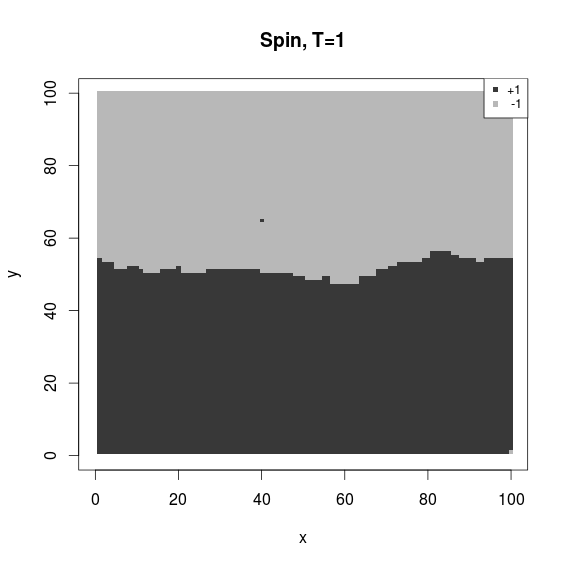
\includegraphics[width=1\linewidth]{spins/spinT1doms}
\end{subfigure}
\begin{subfigure}{.35\textwidth}
  \centering
  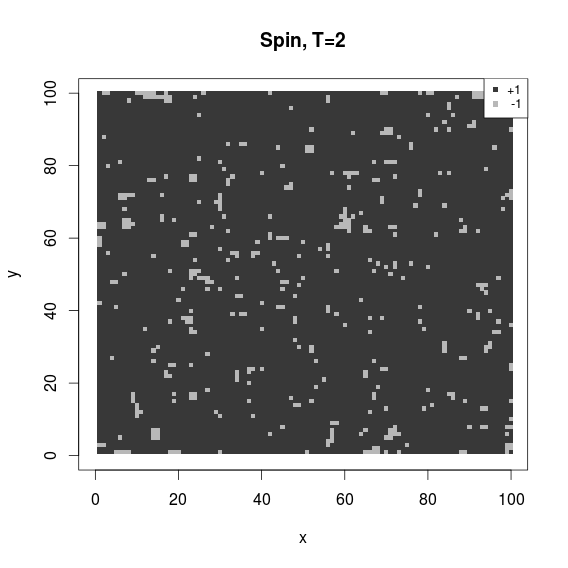
\includegraphics[width=1\linewidth]{spins/spinT2+}
\end{subfigure}%
\begin{subfigure}{.35\textwidth}
  \centering
  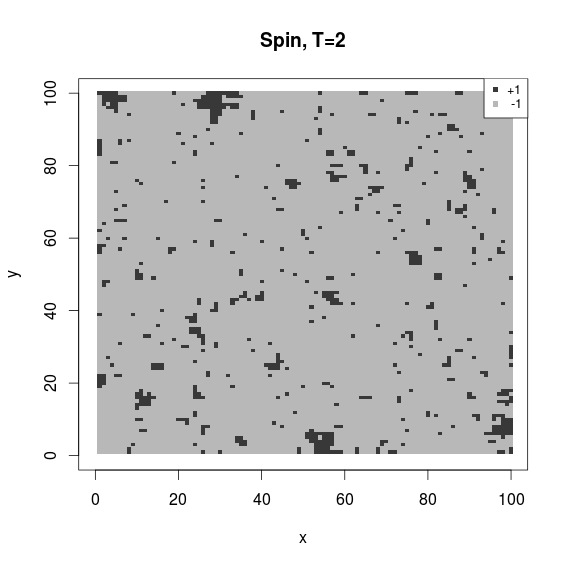
\includegraphics[width=1\linewidth]{spins/spinT2-}
\end{subfigure}%
\begin{subfigure}{.35\textwidth}
  \centering
  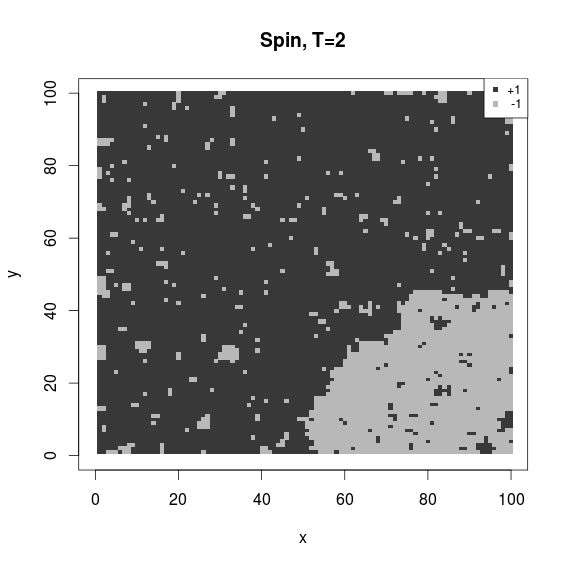
\includegraphics[width=1\linewidth]{spins/spinT2doms}
\end{subfigure}
\begin{subfigure}{.35\textwidth}
  \centering
  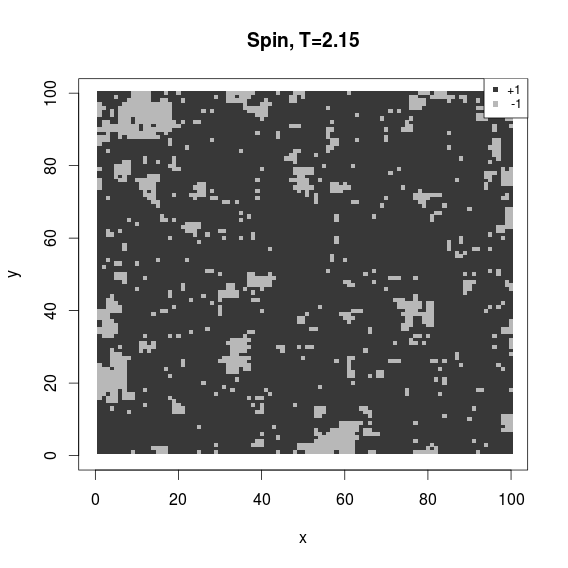
\includegraphics[width=1\linewidth]{spins/spinT2_15}
\end{subfigure}%
\begin{subfigure}{.35\textwidth}
  \centering
  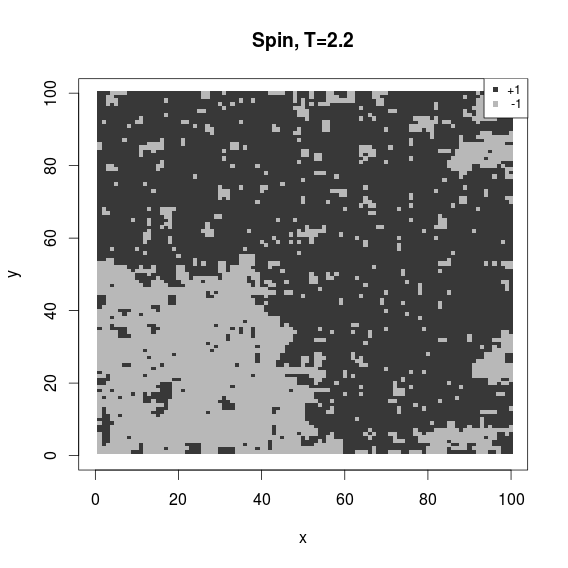
\includegraphics[width=1\linewidth]{spins/spinT2_2}
\end{subfigure}%
\begin{subfigure}{.35\textwidth}
  \centering
  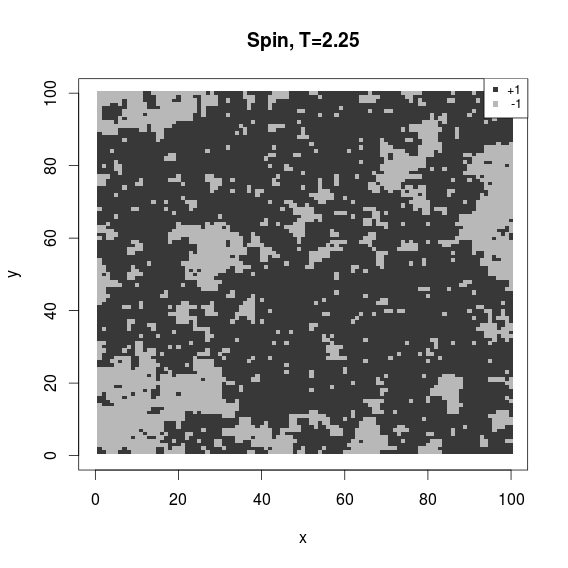
\includegraphics[width=1\linewidth]{spins/spinT2_25}
\end{subfigure}
\caption{Evolución temporal de la magnetización media para diferentes temperaturas alejadas de $T_c$, representando en cada caso todos los comportamientos que pueden darse.}
\label{fig:spinsTc}
\end{figure}

\end{document}